\chapter{Introduction}\label{chap:introduction}

  \section{Overview}\label{sec:overview}

    As founder and CEO of Uber, Travis Kalanick is an example of a resilient leader~\parencite{aib2015}, who stands by his principles and is comfortable with negotiation~\parencite{bhattacharya2015}. Kalanick has demonstrated on countless occasions that as an entrepreneur, he always tries to push the limits~\parencite{smith2014}, further reinforcing his risk-taking behaviour and mind-set. However, a recent scandal involving Uber's senior vice president Emil Michael raised the question of whether Kalanick's approach to leadership had fostered an insensitive, thuggish, hyper-aggressive culture within the organisation. Michael proposed that Uber start spying on journalists to dig up dirt on the personal lives of journalists who wrote negatively about the company~\parencite{withnall2014} in response to an article which highlighted the overt sexism and misogyny that Uber appeared to embrace, with direct regard to Kalanick's gross public comments that his company should be called ``Boober'' because of the sexual attention he gets, as a result of Uber's continued growth and success~\parencite{lacy2014}. 

    \begin{figure}
      \centering
      \begin{minipage}{7cm}
        \centering
        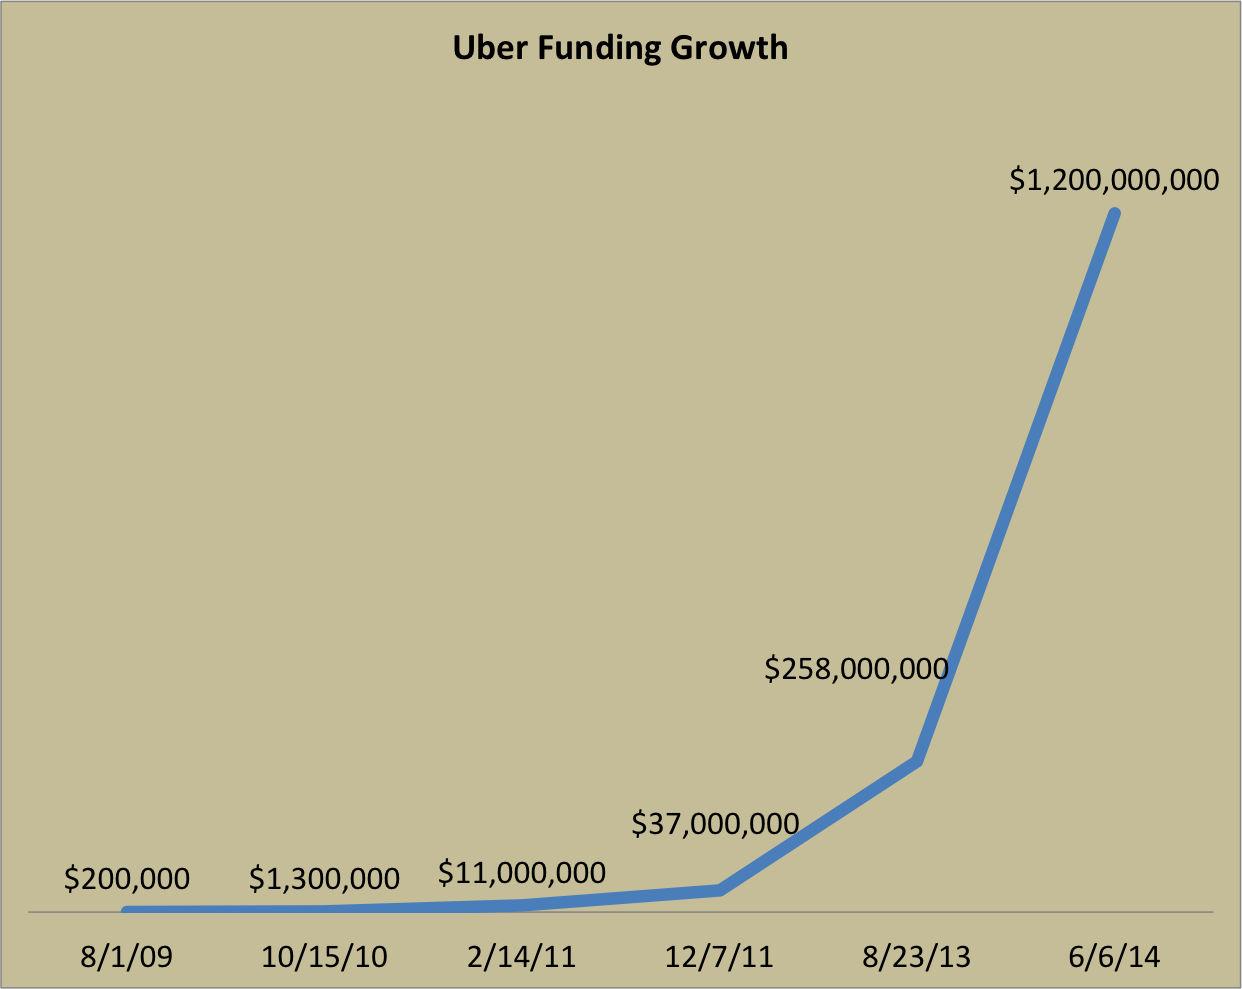
\includegraphics[width=7cm]{inc/uber_funding_growth.png}
        \caption[Uber Funding Growth]{Uber Funding Growth~\parencite{ferenstein2014}}
        \label{fig:uber_funding_growth}
      \end{minipage}
    \end{figure}

    Despite Kalanick's misgivings, Uber continues to grow exponentially see Figure~\ref{fig:uber_funding_growth}, recently completing a new round of funding that values the five-year-old company at close to \$51 billion~\parencite{macmillan2015}. An appraisal of Kalanick's leadership credentials is necessary in order to determine his contribution to the company's success. Consequently, the focus of this section is Uber's founder and CEO, Travis Kalanick -- specifically, the characteristics which assert his title as an entrepreneur. As this term ``entrepreneur'' is relevant to multiple academic contexts, such an appraisal will need to be espoused from models stemming from the fields of psychology, economics and sociology.

  \section{Psychological Conceptions}\label{sec:psychological_conceptions}

    Psychologists tend to focus on aspects of the entrepreneur's personality, viewing them as an individual who is typically driven to experiment, perform and succeed. In addition, by starting to work on their own, entrepreneurs gain the independence required to make their own decisions~\parencite{groenewald2006}. Kalanick demonstrated such traits at an early stage when starting his first company, Scour.com, a peer-to-peer search engine which could find media content on the internet~\parencite{kessler2013}. Shortly after launching in 1998, Scour.com faced two major lawsuits over copyright infringement~\parencite{huffstutter2000}, and as the company was not able to raise money to continue operations, it filed for bankruptcy protection in order to protect itself from the impending lawsuits.

    Unperturbed by the occasion, Kalanick quickly moved on to start Red Swoosh in 2001, a relatively unsuccessful peer-to-peer file sharing company which he subsequently sold to Akamai for \$15 million in 2007. Long-term investors in Red Swoosh, asserted that Kalanick was focused, tireless and never revealed a loss of faith during this period, a testament to his hardiness~\parencite{mishkin2015}. Hardiness is a personality characteristic which is resistant to stress~\parencite{kobasa1979}. According to Cardwell \& Flanagan~\parencite{cardwell2008}, hardy individuals such as Kalanick demonstrate three characteristics:

    \begin{enumerate}
      \item Control of their lives.
      \item A strong sense of purpose combined with involvement in the world around them.
      \item A view that challenges are an opportunity to overcome and develop rather than threats or stressors.
    \end{enumerate}

    \begin{figure}
      \centering
      \begin{minipage}{7cm}
        \centering
        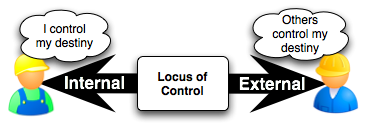
\includegraphics[width=7cm]{inc/locus_of_control.png}
        \caption[Locus of Control ]{Locus of Control~\parencite{shead2007}}
        \label{fig:locus_of_control}
      \end{minipage}
    \end{figure}

    Kalanick's positive reaction to his initial failures demonstrates that he had an internal locus of control~\parencite{rotter1966}, which was complemented by a high sense of self-efficacy~\parencite{bandura1994}. Individuals with an internal locus of control have a stronger belief that they can control their own environment, and will be more likely to exploit an entrepreneurial opportunity compared to people with an external locus of control~\parencite{engler2009}. However this requires a supplementary belief -- self-efficacy, which reflects ``confidence in the ability to exert control over one's own motivation, behaviour, and social environment''~\parencite{carey2015}. Furthermore, self-efficacy is characterised by being assured that one will accomplish a particular goal -- and to expand on this in a more present context, it can be supported by how Kalanick confidently speaks of Uber aim's to ``push rates so low that Uber rides could be a viable alternative to owning car, and possibly using public transport''~\parencite{mishkin2015}.

  \section{Economic Conceptions}\label{sec:economic_conceptions}

    \begin{figure}
      \centering
      \begin{minipage}{8cm}
        \centering
        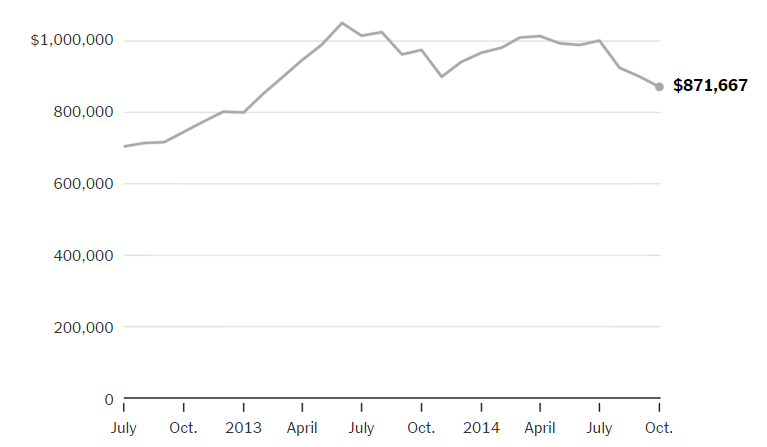
\includegraphics[width=8cm]{inc/new_york_city_taxi_medallion_prices.png}
        \caption[New York City Taxi Medallion Prices]{New York City Taxi Medallion Prices~\parencite{barro2014}}
        \label{fig:new_york_city_taxi_medallion_prices}
      \end{minipage}
    \end{figure}

    Kalanick is a model ``Schumpeterian'' entrepreneur, having disrupted the transportation service industry with the creation of Uber's smartphone app -- an innovative offering which uses GPS technology to match customers with nearby private drivers, then allows them to track the journey in real time from beginning to end, and pay the fare without ever having to reach into their wallets~\parencite{gatehouse2015}. Schumpeter's entrepreneur is an agent of change, which brings about creative destruction through the introduction of new products, processes and services -- upsetting the conventional manner of doing things. For instance in this context, to own a taxi in New York, you require a medallion, a city-issued licence which is required in order to legally pick up passengers flagging on the street. However, since the inception of Uber, taxi medallion prices have been falling in major cities throughout the United States (cf.\ Figure~\ref{fig:new_york_city_taxi_medallion_prices}), due to Kalanick's increasing workforce of private drivers. Kalanick claims that Uber neither own nor operate a taxi service, therefore the company's private drivers, which are employed as contractors, do not have to adhere to regulations.

    \begin{figure}
      \centering
      \begin{minipage}{10cm}
        \centering
        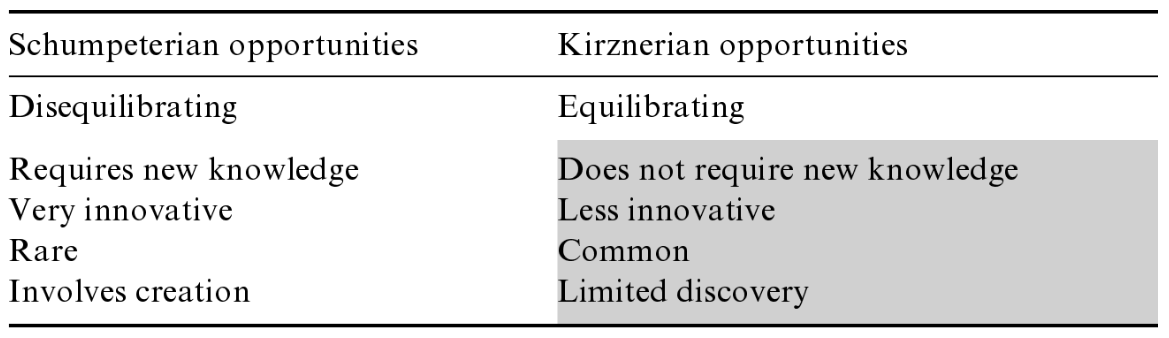
\includegraphics[width=10cm]{inc/opportunity_recognition.png}
        \caption[Opportunity Recognition]{Opportunity Recognition}
        \label{fig:opportunity_recognition}
      \end{minipage}
    \end{figure}

    Unlike Schumpeter's entrepreneur, a creator of disequilibrium in the market --\parencite{kirzner1973entrepreneurship} saw the entrepreneur as a seeker of imbalances, which they aim to remove by means of their entrepreneurial activity see Figure~\ref{fig:opportunity_recognition}. Kirzner's entrepreneur does not create anything new, but simply recognises and exploits what is already there, which others are not aware of~\parencite{landstrom2010entrepreneurship}. In a recent interview with The Wall Street Journal newspaper~\parencite{kessler2013}, Kalanick recalls a conversation with Garrett Camp in 2007, in which Camp said: ``I just want to push a button and get a ride. Travis, let's go buy 10 Mercedes S-Classes, let's go hire 20 drivers, let's get parking garages and let's make it so us and a 100 friends can push a button and an S-Class would roll up, for only us, in the city of San Francisco, where you cannot get a ride. This wasn't about building a huge company, this was about us and our hundred friends''. From this, Kalanick became alert to the opportunity that he could also recruit limousine drivers not on a call. Instead of idly waiting for work, they could pick up and drop off potential customers in the local area. Afterwards, Kalanick went on to employ private drivers, which were vetted by Uber, in order to meet growing demand. Like Kirzner's entrepreneur, Kalanick was able to identify market ignorance with respect to a certain opportunity and act on it~\parencite{hindle2011handbookofresearch}.

    In the case of Kalanick, there is a strong argument for integrating both the Schumpeterian and Kirznerian perspectives in order to appreciate that Uber's success is a result of technology and product oriented disruptive innovation (Schumpeterian) and market oriented strategy (Kirznerian). Without an intersection of the two views, Kalanick would not have succeeded as an entrepreneur.

  \section{Sociological Conceptions}\label{sec:sociological_sonceptions}

    It could be argued that certain subtleties of Kalanick's entrepreneurial characteristics are socially embedded. \cite{reynolds1991} asserts that sociological background is one of the decisive ``push'' factors to become an entrepreneur -- e.g.\ marginalised groups overcome all obstacles and strive for success to make life better, spurred on by their disadvantaged backgrounds~\parencite{simpeh2011}.

    An entrepreneur can complement their business resources by relying on their contacts. The contacts that lead to successful outcomes form part of their ``social capital'', and become a key component of their entrepreneurial networks~\parencite{burt1995}. As noted in section~\ref{sec:economic_conceptions}, Kalanick's conversations with Camp, an entrepreneur who at the time had just sold his company ``StumbleUpon'' to eBay for \pounds75m~\parencite{gonzalez2007}, led to the launch of Uber. From these discussions, it can be asserted that Kalanick talked about the possibility of starting a business with close contacts, as he did not want his intentions to be immediately made public, in case he later perceived that he took that the wrong course of action. This narrative provides a useful bridge to the Knightian theory of entrepreneurship, which focuses on the entrepreneur's role in an ambiguous environment. As the presence of uncertainty requires Kalanick to bear the burden of incorrect decisions, he exercises caution early on, allowing him to tolerate any imminent risks. Moreover, Kalanick's approach gives primacy to the nature of his interaction with the environment -- in lieu with the motivation phase in~\parencite{wilken1979} stage theory.

    \begin{figure}
      \centering
      \begin{minipage}{14cm}
        \centering
        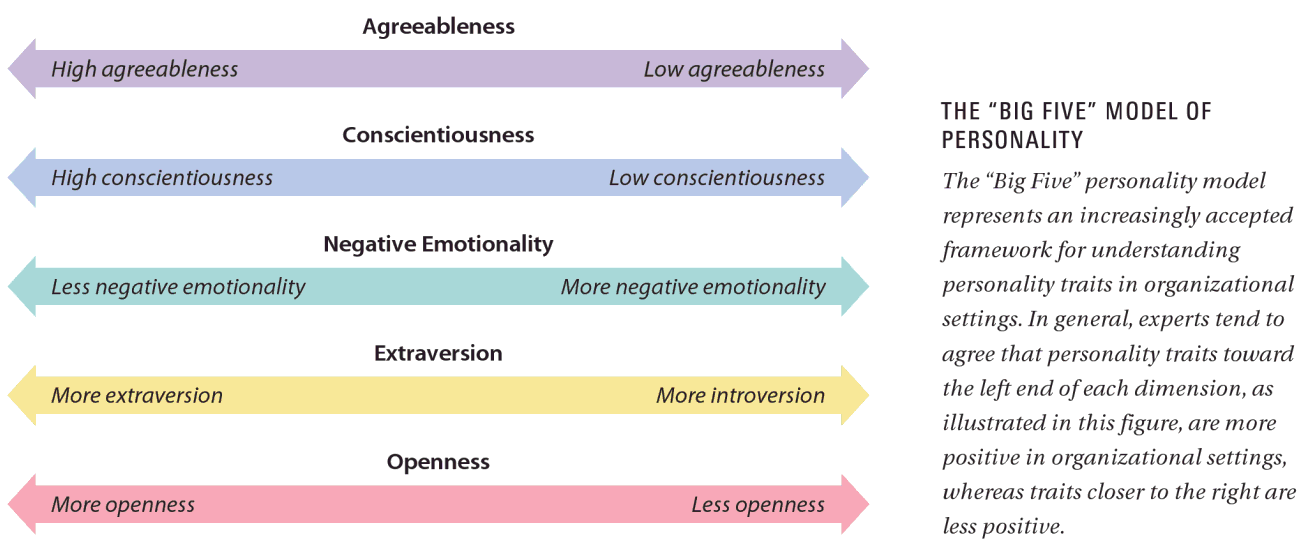
\includegraphics[width=14cm]{inc/the_big_five_model_of_personality.png}
        \caption[The Big Five Model of Personality]{The Big Five Model of Personality}
        \label{fig:the_big_five_model_of_personality}
      \end{minipage}
    \end{figure}

    According to~\parencite{obschonka2013} -- The regional distribution and correlates of an entrepreneurship-prone personality profile in the United States, Germany, and the United Kingdom: A socioecological perspective. The entrepreneurial profile of personality traits in Figure~\ref{fig:the_big_five_model_of_personality}, can be geographically clustered, as it correlates to a higher rate of entrepreneurial activity within a region. 

    \begin{figure}
      \centering
      \begin{minipage}{7cm}
        \centering
        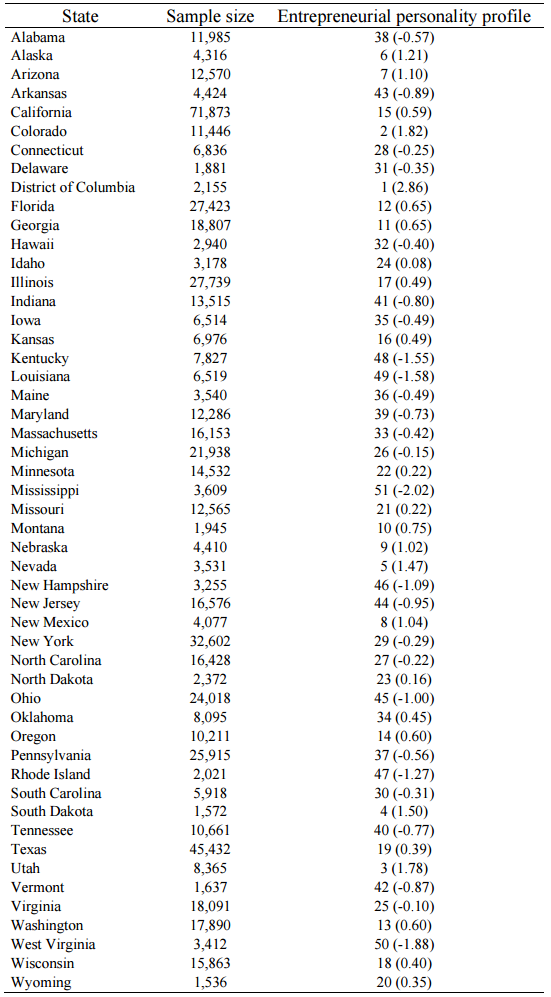
\includegraphics[width=7cm]{inc/entrepreneurship_profile_state_ranking.png}
        \caption[Entrepreneurship Profile State Ranking]{Entrepreneurship Profile State Ranking~\parencite{obschonka2013}}
        \label{fig:entrepreneurship_profile_state_ranking}
      \end{minipage}
    \end{figure}

    The entrepreneurial profile was not as common in less supportive entrepreneurial climates and historically industrial regions (e.g. Indiana and Ohio), as in these areas, the ability to follow rules, not to innovate was valued and considered true success~\parencite{oconnor2013}. With regards to Kalanick’s sociological background, he was raised in California, a state located on the West Coast of the United States. \cite{obschonka2013} concluded that the entrepreneurial trait profile was highest in the West and South, citing historical migration patterns in the U.S.\ as a possible reason. According to \cite{rentfrow2008}, it could have been the more entrepreneurial early settlers who ventured from the East Coast. However, this perspective raises questions about the heritability of personality traits.

  \section{Disadvantages of the Trait-Focused Approach}\label{sec:disadvantages_of_the_trait-focused_approach}

    A trait-focused approach (cf.\ Figure~\ref{fig:entrepreneurship_profile_state_ranking}) to entrepreneurship fails to take situational contexts into account, which is important as some individuals have the traits to help them emerge as entrepreneurs, but not the traits that allow them to become successful entrepreneurs. As determined in section~\ref{sec:sociological_sonceptions}, there can be a number of sociological and situational factors which directly influence entrepreneurship, so it is difficult to have a list of traits in isolation to the context in which the entrepreneurial activity occurs.
